% !TEX encoding = UTF-8
% !TEX TS-program = pdflatex
% !TEX root = ../Tesi.tex
% !TEX spellcheck = en-EN

%************************************************
\chapter{Motivation and Insufficiency of the State of the Art}
\label{cap:insufficiency}
%************************************************

% As already mentioned in \ref{sec:metallurgical industry}, this work focused on
% the particles handled by metallurgical industries.
% \improvement{list of metallurgical processes with particulate materials. E.g.,
% blast furnace is fed with coke and sintered iron ore particles: distribution of
% the feed by the chute, raceway formation} 
% \improvement{More words on motivation:
% industrial processes.
% 1)Ask MB brochure on sinter cooler. 2) Ask TL and CF material on raceway (cite Alice's thesis).} 

\citet{RefWorks:195} states that the iron metal can be obtained by reduction of
iron oxides, of which hematite and magnetite are the most common types. The most
used apparatus to obtain pig iron is the blast furnace.
Iron oxides are mined from earth crust. 
However, a blast furnace needs particles
ranged between 7 and 25 millimiters \cite{RefWorks:195}, to grant a regular
descent of the particle into its hearth.
To reach the required specification, the
extracted minerals are crushed and then sieved. 
Sieving divides the particles in two categories:
\begin{itemize}
  \item{lump ore, between 7 and 25 millimiters,}
  \item{fines, less than 7 millimiters.} 
\end{itemize}

\begin{figure}[!htb]
\centering
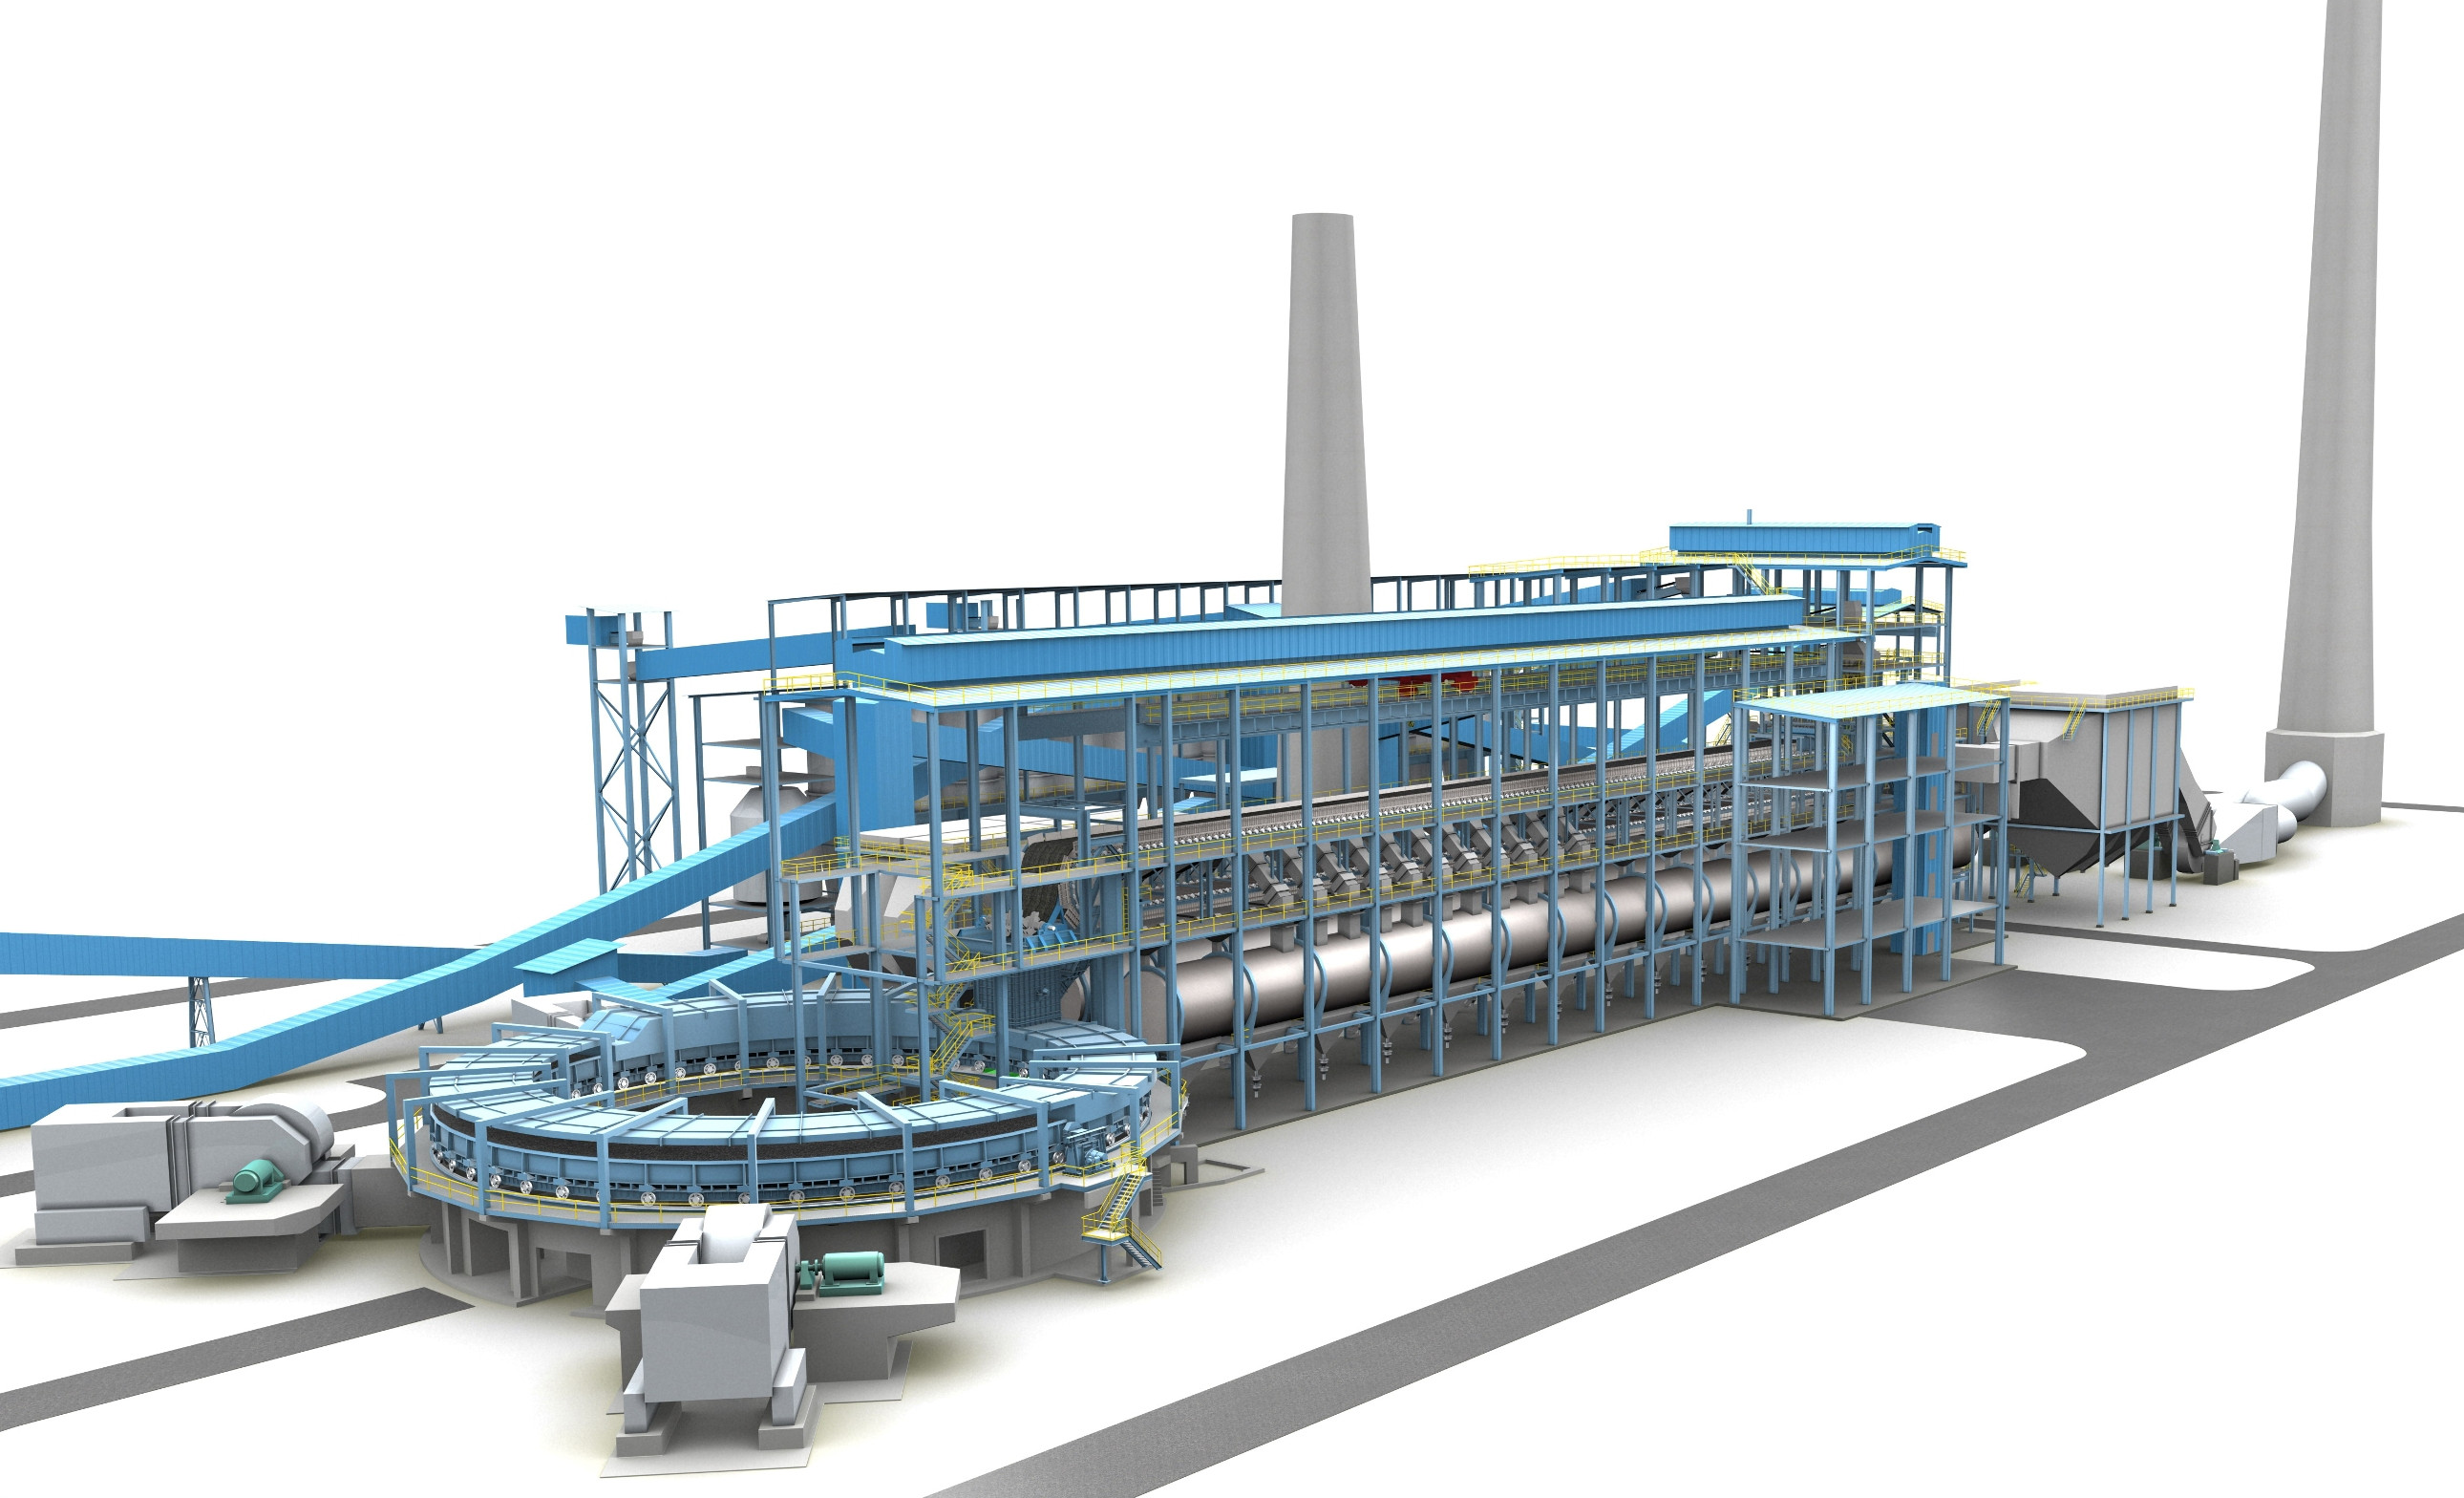
\includegraphics[width=.92\columnwidth]{images/124sinterplant}
\caption[Sinter plant]{Sinter plant (Primetals GmbH).}
\label{fig:124sinterplant}
\end{figure}

Lump ore can be used directly for blast furnace smelting. 
Instead, fines need to be sintered (Fig. \ref{fig:124sinterplant}). \\

\section{Sintering}
\label{sec:sintering}

Sintering consists in partially melting the
fines with limestone and coke.\\
The resulting granular material needs nonetheless to be cooled for
transportation and storage. 
The metallurgical industry uses a \textit{sinter chute cooling system} for this
purpose, see Fig. \ref{fig:124sinterplant}, with many phases:
\begin{enumerate}
  \item{Hot particles are fed into a chute, which deposits the
  particles on a rotating system and segregates them, i.e. lays the large
  particles on the bottom and the small ones on top.}
  \item{Air is injected from the bottom of the rotating system, cooling the
  particles.}
  \item{The resulting particles larger than 25 millimiters are crushed, and
  reinserted in the flow.}
  \item{The particles smaller than 7 millimiters are melted once
  more.}
  \item{The particles between 7 and 25 millimiters are ready for blast furnace
  smelting.}
\end{enumerate}

In our thesis, we focused on (1), and the particles involved in this process.\\

\section{Blast furnace}
\label{sec:blastfurnace}

Well explained in the vast literature (\cite{RefWorks:203}), 
iron making consists in separating the iron from its chemical combination with
oxygen. 
As of now, the blast furnace (Fig. \ref{fig:125blastfurnace}) is considered the
most efficient process.
It can be described as a countercurrent heat and oxygen exchanger.
High temperature air, eventually in combination with pulverized coal, is
inserted into the inferior section of the apparatus.\\

\begin{figure}[!htb]
\centering
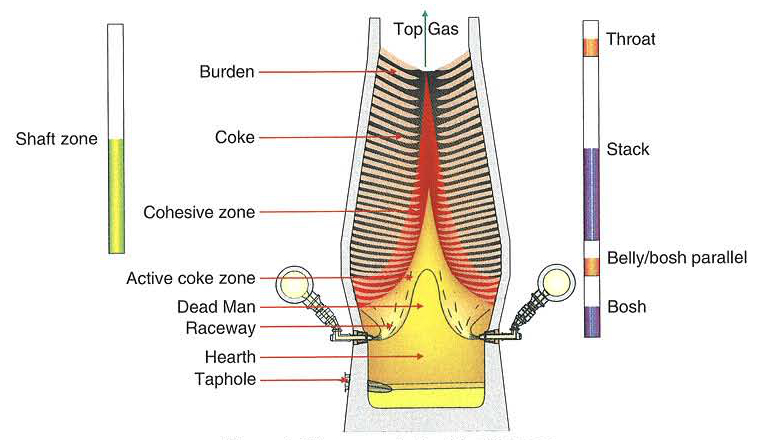
\includegraphics[width=.86\columnwidth]{images/125blastfurnace}
\caption[Blast furnace scheme]{Blast furnace scheme \cite{RefWorks:200}.}
\label{fig:125blastfurnace}
\end{figure}

While rising, the gases
provide the surronding particles with heat, and exits out the superior section
of the furnace.
Symmetrically, iron oxydes descend from the superior section and it is converted
to metallic iron, which is collected into the inferior section.\\

\subsection{Blast furnace structure}
\label{subsec:blastfurnacestructure}

The blast furnace is a massive vertical apparatus, built with consistent amounts
of refractory materials and a robust steel shell.\\
We can divide it in five sections from bottom to top:
\begin{enumerate}
  \item{hearth, where metal and slags are collected and tapped at regular
  intervals;}
  \item{bosh, into which a special type of pipes, called tuyeres, insert the air
  at a temperature between $900^{\circ}$ and $1350^{\circ}$;}
  \item{bosh parallel;}
  \item{stack;}
  \item{throat, where the solid charge of ore and coke is provided, and
  partially exhaust combustion gases exit;}
\end{enumerate}
The areas in front of each tuyere, which can be seen in Fig.
\ref{fig:125blastfurnace}, is called $raceway$ and is the most active. 
We dedicated chapter \ref{cap:blastfurnace} to the investigation of its
behaviour.

\subsection{Blast furnace chemistry}
\label{subsec:blastfurnacechemistry}

The most relevant chemical reactions inside the furnace are presented in Eq.
\ref{eq:co2}.

\begin{equation}
\label{eq:co2}
\begin{aligned}
	2C + O_2 & \rightarrow 2CO + heat, \\
	Fe_2O_3 + 3CO & \rightarrow 2Fe + 3CO_2 .
\end{aligned}
\end{equation}


However, not only the combustion of coke inside the charge provides the heat
necessary for iron melting.
The air provided by the tuyeres is pre-heated through a combination of
recycled exit combustion gases and methane. 

\section{Materials characterization}
\label{sec:materialscharacterization}

A univocal
method to characterize the mentioned particles has so far not been established.
From the experimental point of view, the main issues are the difficult setups and the general 
reliability and reproducibility of the tests. 
From the numerical point of view, no general procedure is available, and the existence of a 
mathematically unique solution describing macro/micro particle contact has yet
to be proved.\\
Moreover, in a recent study, \citet{RefWorks:56} implied "that the dynamic properties of a 
powder cannot be applied to universally predict the static properties of a powder, and, likewise, 
the static properties cannot be used to predict dynamic properties".\\

\section{DEM Simulations}
\label{sec:demsimulations}

Many authors used \acs{DEM}, the discrete
element method used in this work, to understand sintering processes 
\cite{RefWorks:196, RefWorks:197} and smelting \cite{RefWorks:198,
RefWorks:199}.\\
In their original formulation of \acs{DEM} \citet{RefWorks:172} allowed two particles to slightly overlap upon
contact, see Fig. \ref{fig:062collision}, and consequently they proposed
repulsive forces in relation to this overlap distance.
\begin{figure}[!htb]
\centering
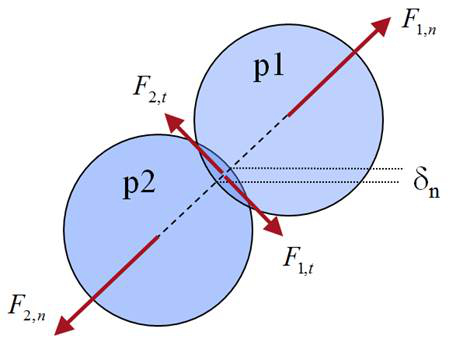
\includegraphics[width=.50\columnwidth]{images/062collision}
\caption[Soft sphere model]{Soft sphere model.}
\label{fig:062collision}
\end{figure}
The force that particle $i$ exerts on particle $j$ is defined as:
\begin{equation}
m \ddot{x}_{ij} + c \dot{x}_{ij} + k x_{ij} =  F_{ij} .
\label{equ:newtonlaw}
\end{equation}

Their fundamental modelling concept of \acs{DEM} has
since been widely accepted in the literature and their soft sphere contact law has been developed further by
numerous researchers (\citet{RefWorks:148} and \citet{RefWorks:145}).
With increasing computational resources, \acs{DEM} simulations have become very
popular giving rise to the development of commercial (e.g., $PFC3D$, used by
\citet{RefWorks:87}) and open-source softwares (e.g.,
\acs{LIGGGHTS}, \citet{RefWorks:136}, \citet{RefWorks:139}).
Soft-sphere \acs{DEM} simulations of thousands of particles have been proven to 
faithfully model particle bulk behaviour, as in Fig. \ref{fig:061cfdemsim}
(\citet{RefWorks:86}).\\
\begin{figure}[!htb]
\centering
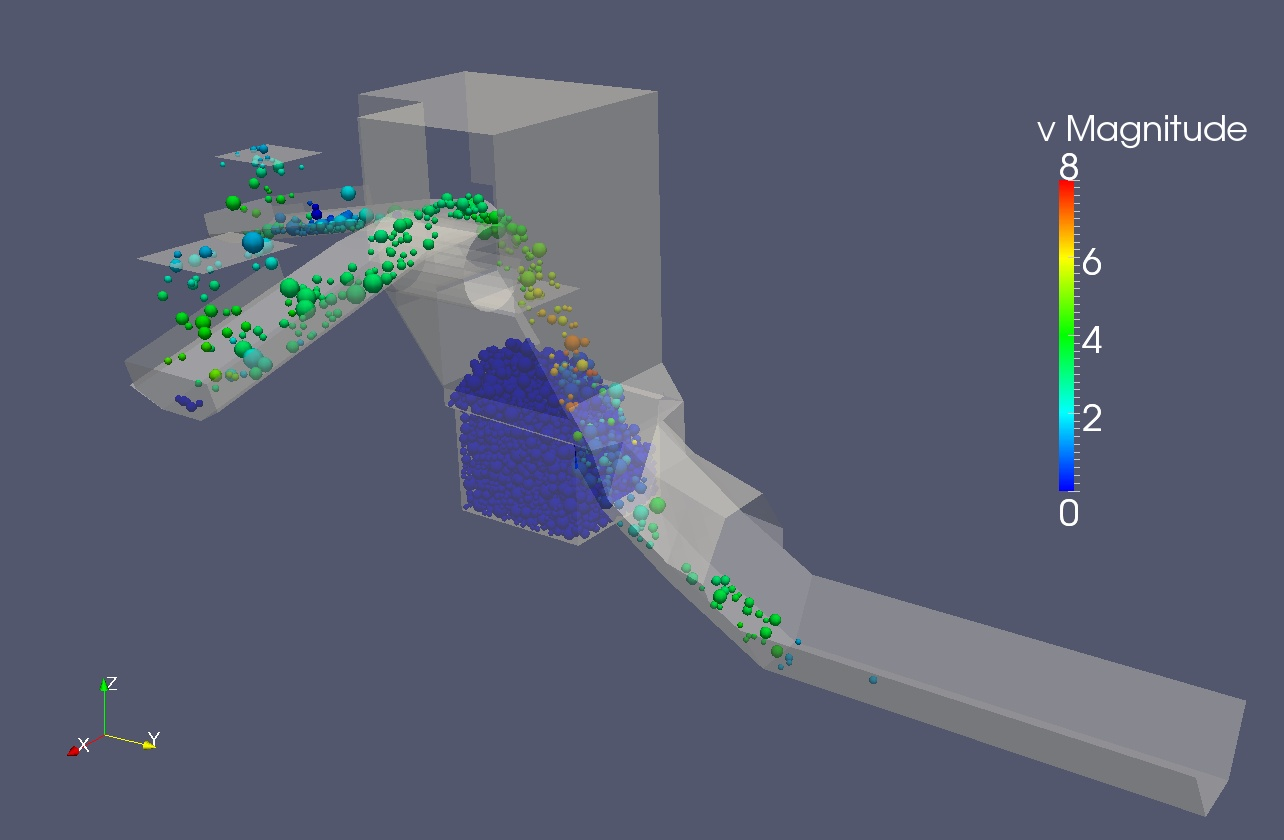
\includegraphics[width=.70\columnwidth]{images/061cfdemsim}
\caption[DEM simulation]{Example of a DEM simulation (www.cfdem.com).}
\label{fig:061cfdemsim}
\end{figure} 

\section{Parameters}
\label{sec:parameters}

In these macroscopic \acs{DEM} simulations, the contact law kernel between a 
pair of particles determines the global bulk behaviour of the granular material
(\citet{RefWorks:131}).
As a consequence, defining a correct contact law is of crucial importance for the predictive 
capability of \acs{DEM} simulations. 
Since \acs{DEM} contact laws are based 
on a set of semi-empirical parameters, correct contact law 
parameters must be defined for a given granular material
or \acs{DEM} simulations will fail (\citet{RefWorks:177}). \\
Identifying \acs{DEM} contact law parameters is not a trivial task. 
Due to the huge number of particles in a granular material, it
may be impractical to identify valid parameter sets by performing bilateral 
particle collision experiments. 
Furthermore, some contact law parameters such as the coefficient of rolling
friction are purely empirical and cannot be determined by direct 
particle-to-particle measurements (\citet{RefWorks:87}).
Therefore, \acs{DEM} contact law parameters (Table \ref{tab:08DEMparameters}) are
commonly determined by comparing the macroscopic outcome of large-scale \acs{DEM}
simulations with bulk experiments (\citet{RefWorks:91}). 
If \acs{DEM} simulation results disagree with bulk measurements, the set of contact
law parameters must be adjusted until reasonable agreement is achieved, as
explained in Section \ref{sec:parametersidentification}.\\
However, this purely forward methodology of parameter identification is limited by 
the multi-dimensionality of the parameter space and the associated computational costs of the required 
\acs{DEM} test simulations. 
Moreover, one parameter set which is valid for one bulk behaviour (e.g., angle
of repose) might fail for another (e.g., shear tester). \\

\subsection{Direct Determination}
\label{subsec:directdetermination}

\begin{figure}[!htb]
\centering
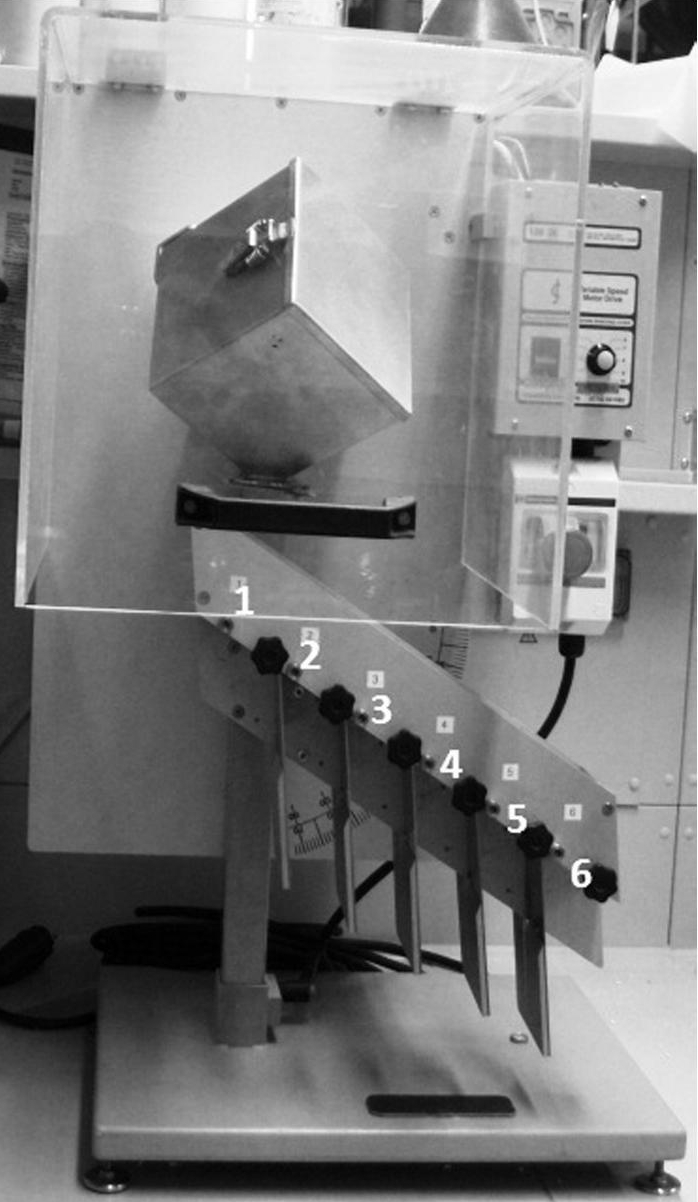
\includegraphics[width=.30\columnwidth]{images/126qpmtester}
\caption[QPM tester]{QPM tester \cite{RefWorks:177}.}
\label{fig:126qpmtester}
\end{figure}
There are yet ways to determine contact parameters directly by measuring
material properties or by performing particle based experiments, see e.g.
\citet{RefWorks:177}, \citet{RefWorks:181}, and \citet{RefWorks:186}, as in
Fig. \ref{fig:126qpmtester}.\\
However, these methodologies are laborious, 
since they have to be performed for every new granular material prior to a \acs{DEM}
simulations. 
Especially for the already cited rolling friction parameter, it is arduous to
link the rolling friction parameter to the non-sphericity of the particle.
In literature (e.g., \citet{RefWorks:177}) is usually desumed from the angle of
repose (\acs{AoR}).
However, in section \ref{sec:pcaanalysis} will be shown how this parameter
accounts only for a portion of the final value.\\
Clearly, there is a
need for an efficient method for identifying \acs{DEM} contact law parameters, given
a specific particle behaviour.



